\documentclass[letterpaper,12pt]{article}
\usepackage[margin=64pt]{geometry}
\usepackage{amsthm}
\usepackage{amsmath}
\usepackage{amssymb}
\usepackage{parskip}
\usepackage{graphicx}
\usepackage{enumerate}
\usepackage{hyperref}
\usepackage{listings}
\newcommand{\transpose}{^{\mbox{\tiny T}}}


\begin{document}
\thispagestyle{empty}

\hrule \vspace{0.5em}
\noindent {\bf CFRM 461: Probability and Statistics for Computational Finance} \hfill Homework 1 \newline \hrule

\begin{enumerate}
\item[Q1.] Features: The median line is closer to the top(Q3), therefore  Q2 - Q1 $>$ Q3 - Q2, the distribution is skewed to the left. The IQR (height of the box) is approximately 10 and there is one outlier at approximately 135.
\item[Q2.] 
\begin{enumerate}
\item[a)]C
\item[b)] A
\item[c)] B
\item[d)] B
\item[e)] C
\item[f)] E
\end{enumerate}
\item[Q3.] 
\begin{enumerate}
\item[a)]
\begin{lstlisting}
> weight <- c(59,70 ,68 ,61, 65, 65, 56, 59, 58)
> height <- c(165 ,191, 183, 173, 173, 165, 152, 157, 178)
> plot(weight,height)
\end{lstlisting}
The plot looks linear, positive, strong
\begin{center}
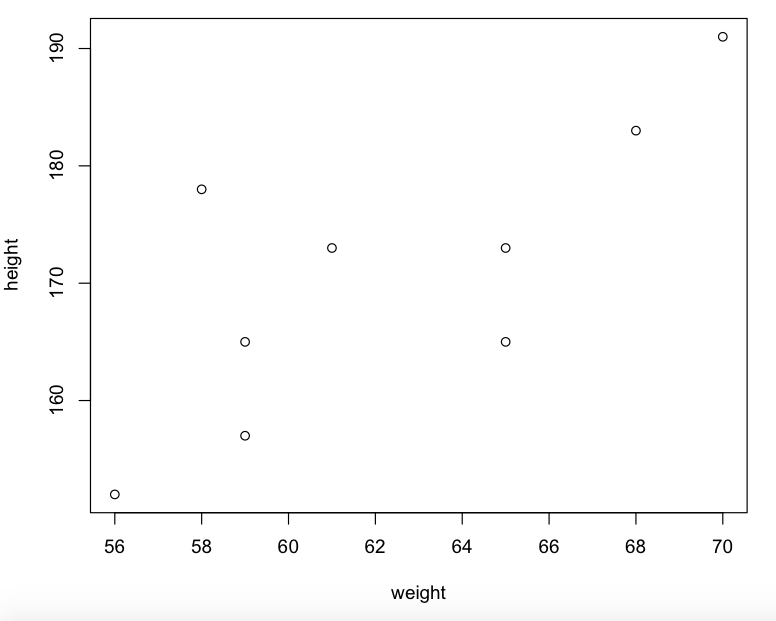
\includegraphics[scale = 0.4]{HW2-Q3-A}
\end{center}
\newpage
\item [b)]
\begin{lstlisting}
> xbar <- mean(weight)
> ybar <- mean(height)
> rho <- cor(weight,height)
> sd_x <- sd(weight)
> sd_y <- sd(height)
> b_1 <- rho*(sd_y/sd_x)
> b_0 <- ybar - b_1*xbar
\end{lstlisting}

y = 49.87 + 1.94x

\item[c)] 49.87 + 1.94(60) = 166.27

\item[d)]
\begin{lstlisting}
> plot(weight,height)
> lines(weight,coef(lm(height~weight))[1] +
coef(lm(height~weight))[2]*weight)
\end{lstlisting}
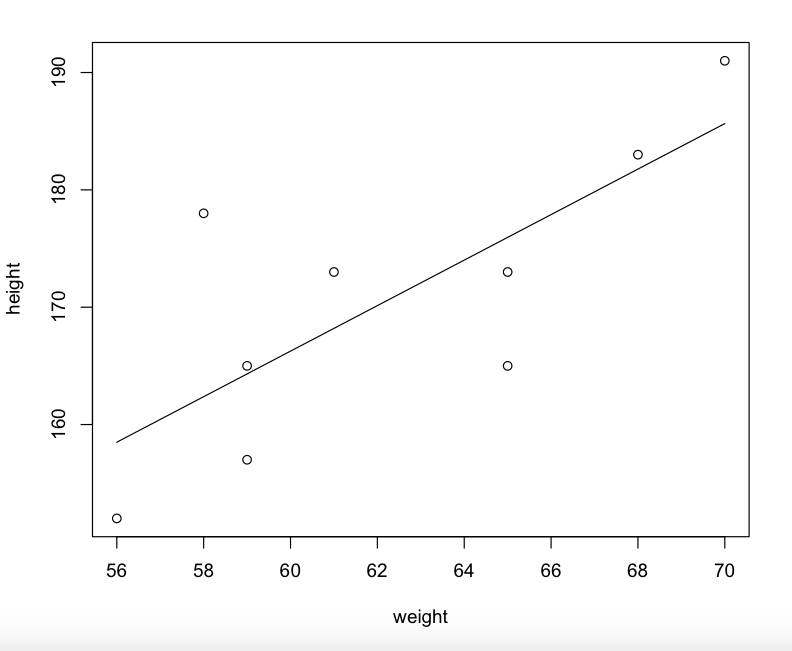
\includegraphics[scale = 0.4]{Plot}
\item[e)]
\begin{lstlisting}
> plot(weight,residual)
> abline(0,0)
\end{lstlisting}
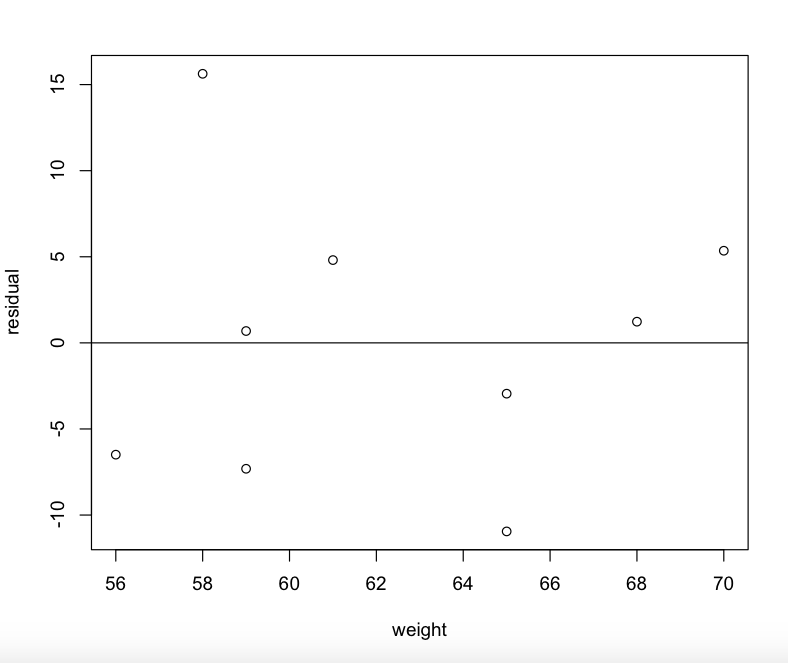
\includegraphics[scale = 0.4]{Resid}\\
The plot looks like there is a random dispersion of points suggesting that a linear model is appropriate. Non-random patterns suggest non-linear relationships. Clearly, this is not the case.
\end{enumerate}
\end{enumerate}

\end{document}